\documentclass[12pt]{article}

\usepackage[utf8]{inputenc}
\usepackage[russian]{babel}
\usepackage{graphicx}
\usepackage{indentfirst}
\usepackage{booktabs}


\graphicspath{{pic/}}

\begin{document}

\begin{center}
	\LARGE 
	\textbf{Практическое занятие 4}\\
	РАБОТА С ГРАФИКОЙ СРЕДСТВАМИ MATLAB\\
\end{center}

\begin{flushright}
	\large
	Игнашов Иван\\
	Вариант 8\\
\end{flushright}

\newpage

 \section*{1. Цель работы}
Изучение основных операторов графики системы MATLAB и создание программ, реализующих графический вывод.
\subsection*{Порядок работы:}
\begin{enumerate}
	\item Составление и отладка программы для вывода графиков функций f1, f2, f3 на основании задания\\
		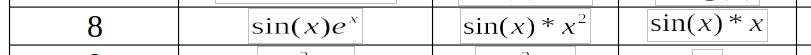
\includegraphics[width=0.75\linewidth]{formula.png}\\
		Вывод графиков должен быть осуществлен в одном окне, графики должны быть подписаны, отмасштабированы.
		
	\item Составление и отладка программы для вывода графика трехмерной поверхности для функции $f4(r = \sqrt{x^2 + y^2}) $ , где f4:\\
		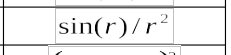
\includegraphics[width=0.4\linewidth]{formula2.png}
	\item Написать файл-функцию для вычисления кусочно-заданной функции и построить ее график\\
		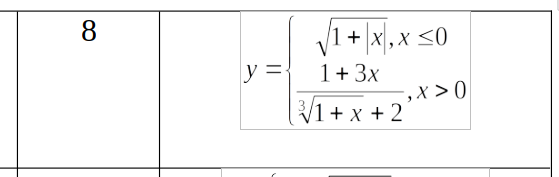
\includegraphics[width=0.75\linewidth]{formula3.png}
\end{enumerate}

\newpage
 \section*{2. Листинг программы для вывода графиков функций}%
 
 \subsection*{2.1. графики f1, f2, f3}
\begin{figure}[!h]
	\centering
	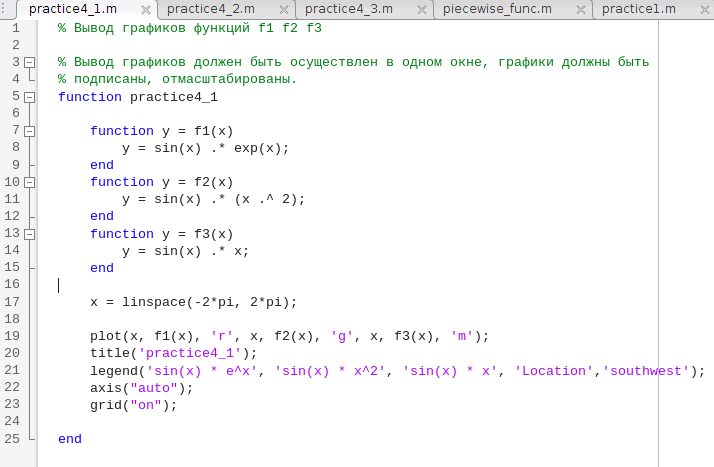
\includegraphics[width=\linewidth]{multiple_lines.png}
	\caption{Программа генерации графиков f1, f2, f3}
\end{figure}
\begin{figure}[!h]
	\centering
	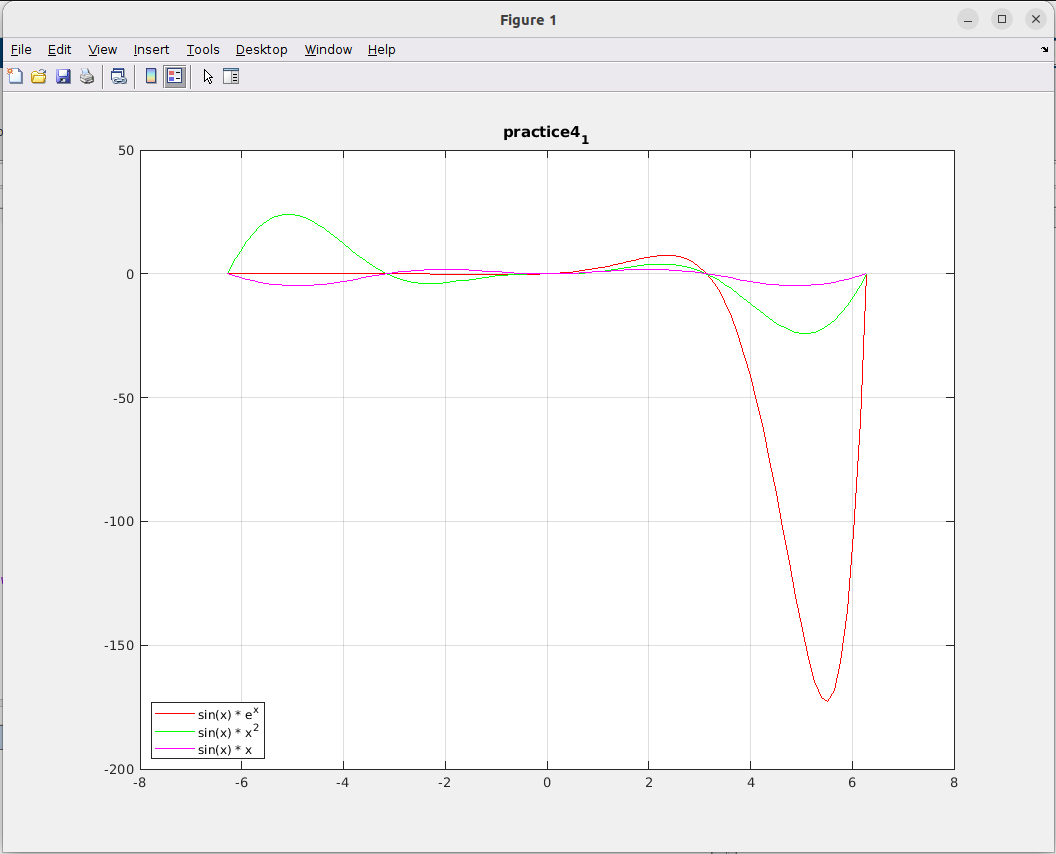
\includegraphics[width=\linewidth]{multiple_lines_plot.png}
	\caption{Графики f1, f2, f3}
\end{figure}
\begin{figure}[!h]
  \subsection*{2.2. трёхмерная поверхность f4}
 \end{figure}

\begin{figure}[!h]
	\centering
	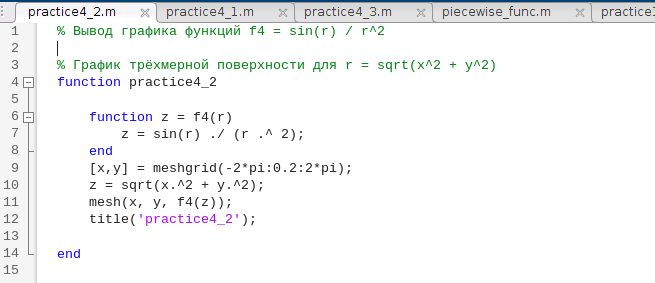
\includegraphics[width=\linewidth]{3d_plot.png}
	\caption{Программа генерации 3D графика f4}
\end{figure}

\begin{figure}[!h]
	\centering
	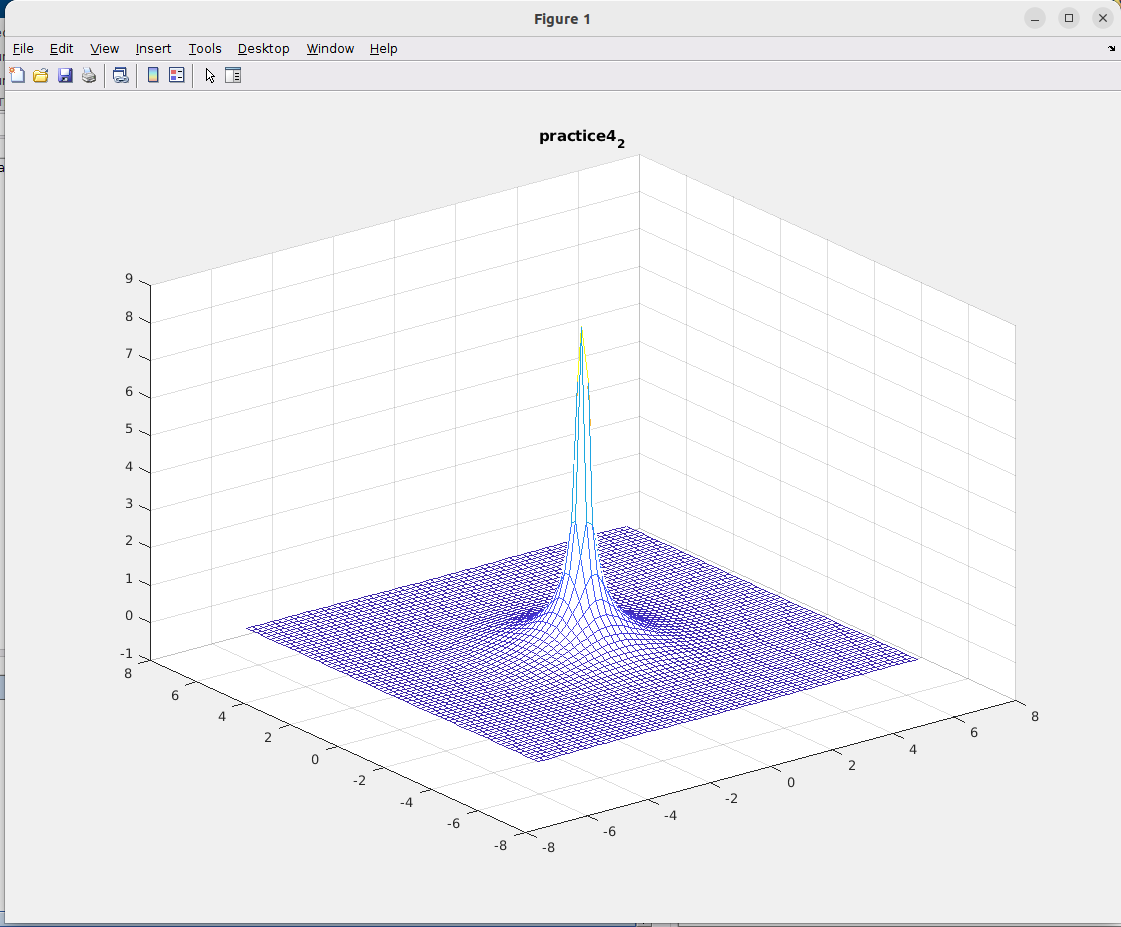
\includegraphics[width=\linewidth]{3d_plot_plot.png}
	\caption{График f4}
\end{figure}
 
 
\begin{figure}[!h]
 \subsection*{2.3. график кусочно-заданной функции} 
\end{figure}
 
\begin{figure}[!h]
	\centering
	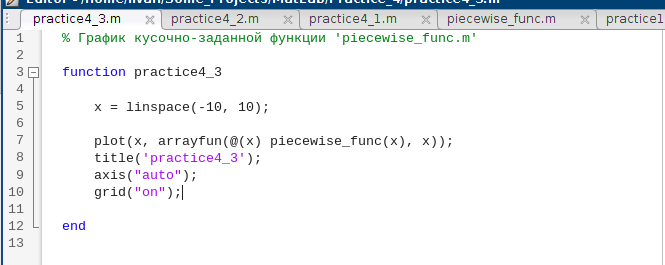
\includegraphics[width=\linewidth]{piecewise_setup.png}
	\caption{Программа генерации графика кусочно-заданной функции}
\end{figure}

\begin{figure}[!h]
	\centering
	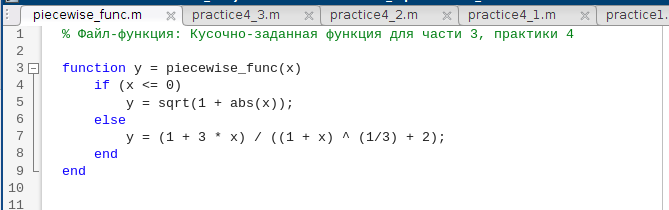
\includegraphics[width=\linewidth]{piecewise_func.png}
	\caption{Кусочно-заданная файл-функция}
\end{figure}

\begin{figure}[!h]
	\centering
	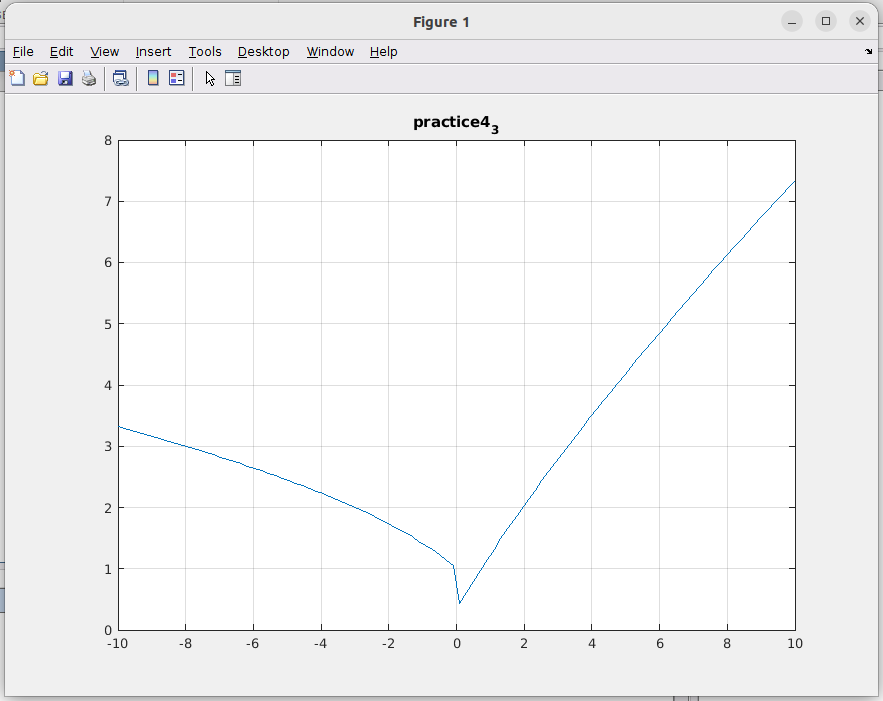
\includegraphics[width=\linewidth]{piecewise_plot.png}
	\caption{График кусочно-заданной функции}
\end{figure}
\end{document}